% !TEX encoding = UTF-8
% !TEX TS-program = pdflatex
% !TEX root = ../tesi.tex

%**************************************************************
\chapter{Contesto aziendale}
\label{cap:introduzione}
%**************************************************************

%**************************************************************
\section{Lab Network}

\begin{figure}[H]
	\begin{center}
	
\includegraphics[scale=0.4]{immagini/LOGO_LABNETWORK.png}
	\caption{Logo \lab{}}
	\end{center}
\end{figure}

\lab{} nasce nel 2016 con lo scopo di aiutare le imprese a creare e ad innovare prodotti e processi attraverso la competenza concreta dei laboratori, sfruttando le potenzialità dei moderni strumenti digitali.\\
Nel dettaglio \lab{} offre la possibilità di importanti avanzamenti tecnologici a PMI offrendo servizi di consulenza oltre che ricerca e sviluppo di progetti sperimentali.\\
L'azienda cerca di collaborare con più partner per poter ottenere una visione maggiore di prodotti e di conseguenza soddisfare i clienti.\\
L'ambiente lavorativo è condiviso con un'altra azienda: \textit{Business Research Srl}, la quale si occupa di soluzioni software su misura, applicazioni per aziende, e-commerce, cloud e hosting.\\
Tra le due aziende è in vigore un accordo che le lega in una stretta collaborazione: infatti, nel periodo di sviluppo di un nuovo progetto, Business Research si occupa della parte software.\\
Durante lo stage ho di fatto interagito con il personale di quest'ultima azienda per la realizzazione del progetto.

\section{Organizzazione aziendale}

\subsection{Processi aziendali}
Al fine di raccogliere l'interesse e sensibilizzare le PMI verso un percorso di aggiornamento tecnologico, l'azienda ha sviluppato uno schema che si divide in tre fasi:
\begin{itemize}
\item Creare l'interesse attraverso politiche di marketing discutendo di temi specifici ad alto impatto mediatico;
\item Raccogliere gruppi omogenei che condividono l'interesse ad una specifica tecnologia;
\item Attraverso attività di consulenza e formazione si cerca da un lato di capire le esigenze produttive e dall'altro le potenzialità che una digitalizzazione (hardware o software) può contribuire alla crescita di una PMI.
\end{itemize}
Dal momento in cui una PMI decide di investire in un aggiornamento tecnologico attraverso l'introduzione di un nuovo prodotto o servizio, \lab{} per prima cosa sviluppa un piano di lavoro che, a seconda delle esigenze del cliente, può prevedere una prima fase di ricerca per passare poi allo sviluppo vero e proprio.\\
Nella fase di ricerca \lab{} coinvolge varie aziende specializzate creando così una rete di imprese che collaborano per portare a termine il progetto innovativo oggetto della ricerca.

\subsection{Metodo di lavoro}
A seguito di una valutazione della complessità del progetto, in collaborazione con Business Research, viene formato un team che seguirà lo sviluppo del progetto dall'inizio alla fine.
Durante i processi di sviluppo di un nuovo progetto vengono seguiti i principi della metodologia agile, ciò consente di avere un dialogo continuo con il cliente che può decidere di modificare il progetto in corso d'opera.
\begin{enumerate}
\item \textbf{Gli individui e le interazioni più che i processi e gli strumenti.}
\item \textbf{Il software funzionante più che la documentazione esaustiva.}
\item \textbf{La collaborazione col cliente più che la negoziazione dei contratti.}
\item \textbf{Rispondere al cambiamento più che seguire un piano.}
\end{enumerate}

\begin{figure}[H]
	\begin{center}
	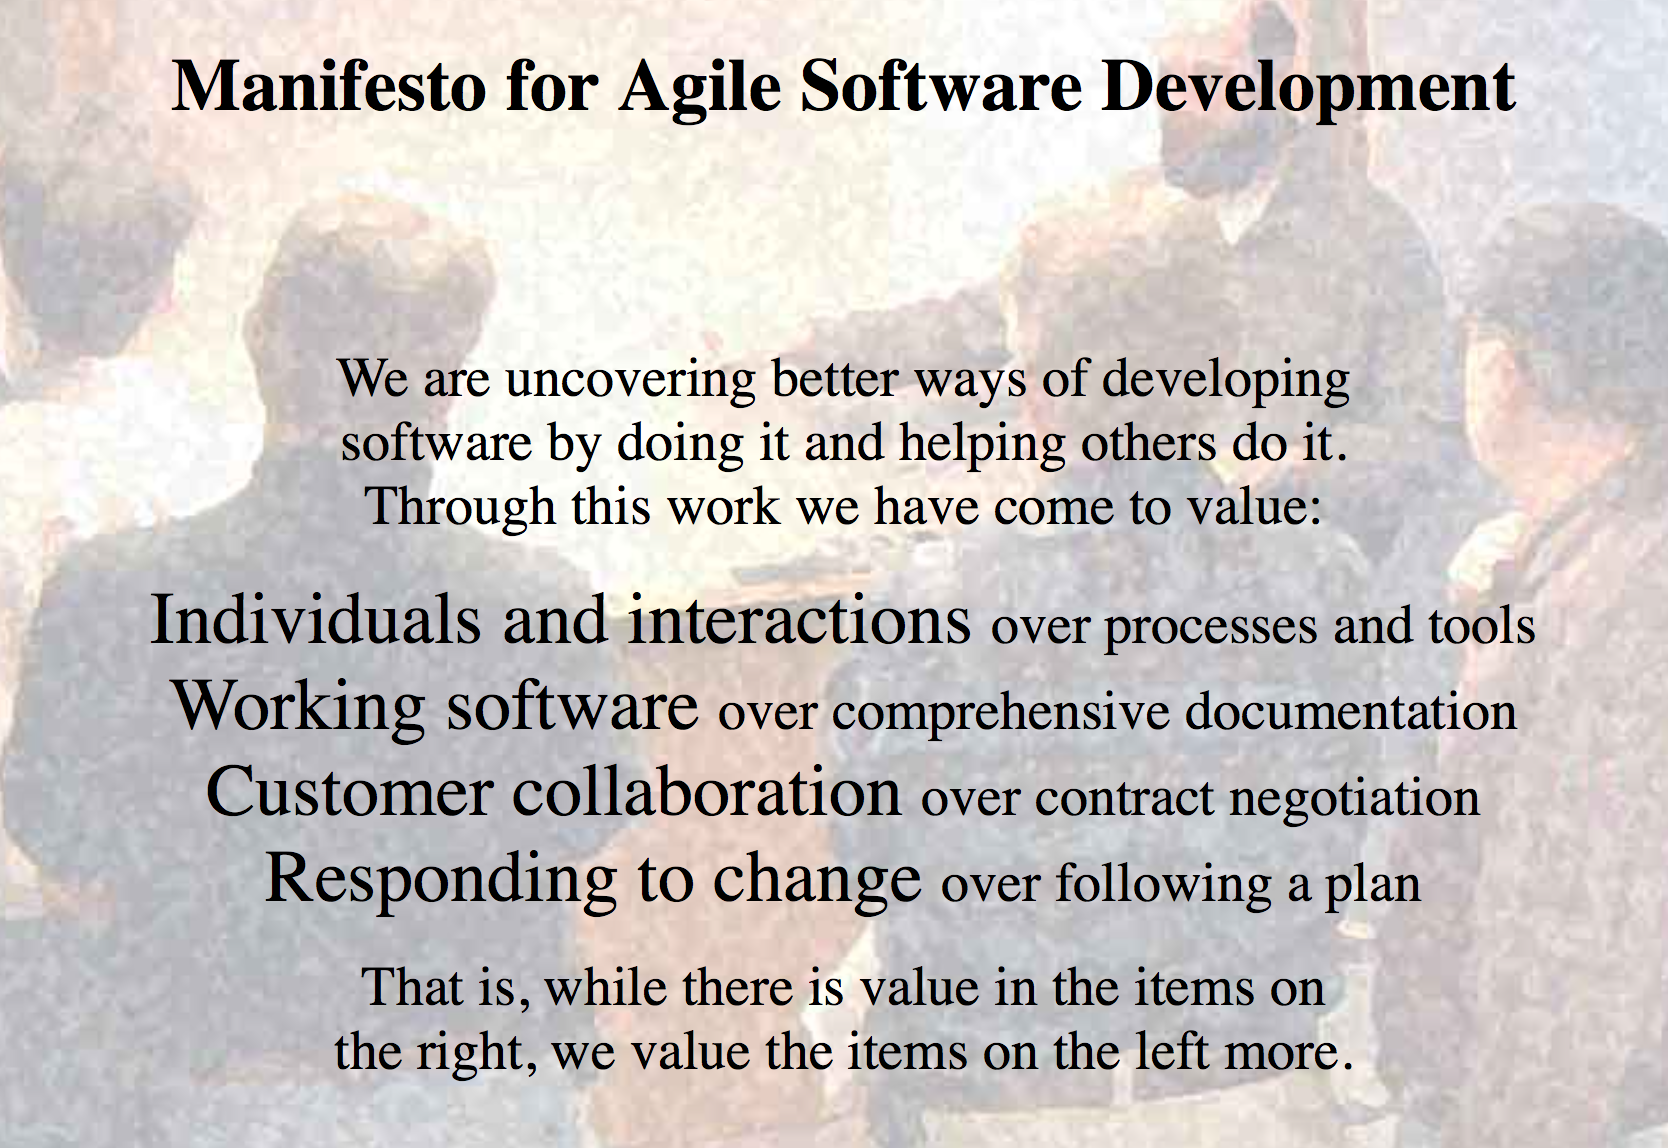
\includegraphics[scale=0.25]{immagini/agile_manifesto.png}
	\caption{I principi del manifesto agile}
	\small{\textbf{Fonte:} \url{http://agilemanifesto.org}}
	\end{center}
\end{figure}

\noindent Il team utilizza il framework \textit{Scrum} per la gestione del ciclo di sviluppo del progetto.
Tale framework definisce i ruoli e il lavoro all'interno del team, denominato quindi \textit{Team Scrum}.\\

\begin{figure}[H]
	\begin{center}
	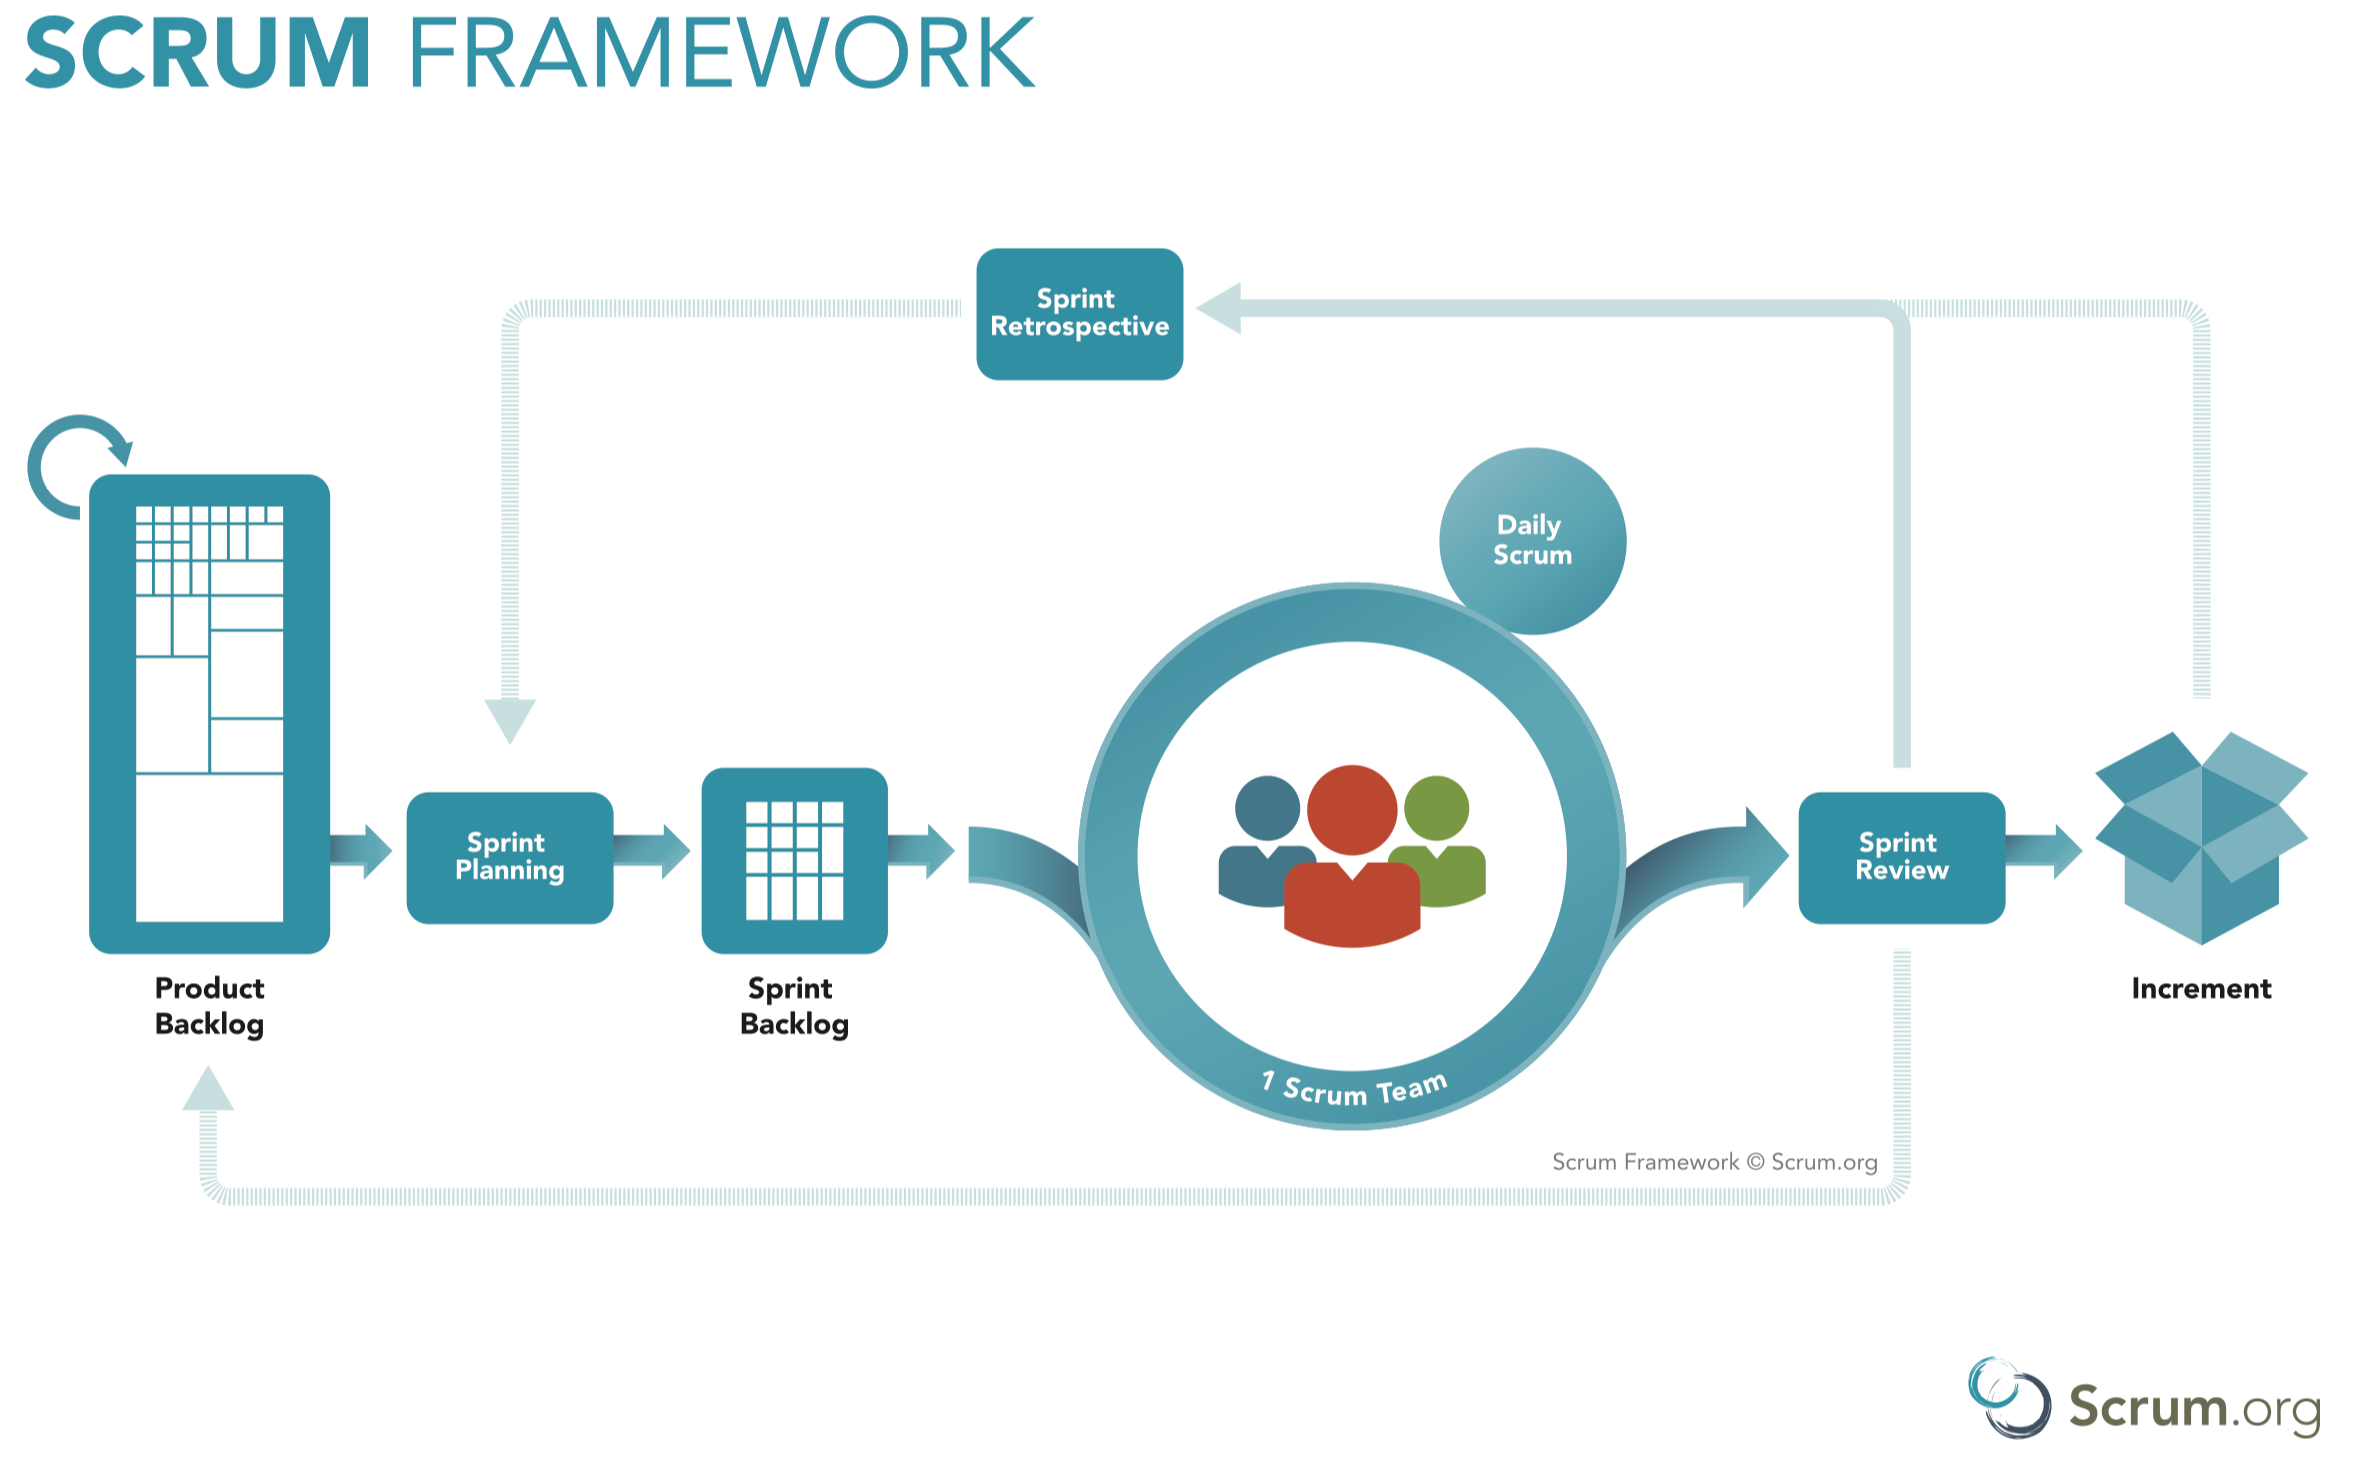
\includegraphics[scale=0.3]{immagini/scrum.png}
	\caption{Schema rappresentativo del framework Scrum}
	\small{\textbf{Fonte:} \url{https://www.scrum.org/}}
	\end{center}
\end{figure}

\noindent \textbf{Team Scrum}\\
\\
Il Team Scrum è composto principalmente da: 
\begin{itemize}
\item \textbf{Product Owner}: può essere definito come il portavoce del cliente, rappresenta gli stakeholders;
\item \textbf{Team di sviluppo (Development team)}: è il team responsabile dello sviluppo del prodotto ed è autosufficiente dal punto di vista organizzativo;
\item \textbf{Scrum Master}: è il ruolo responsabile della risoluzione dei problemi che ostacolano il lavoro del team.
\end{itemize}

\noindent Particolarmente importanti nell'utilizzo di questo framework sono gli aspetti temporali:

\begin{itemize}
\item \textbf{Sprint}: è un'unità di tempo, fissato generalmente tra una e quattro settimane, che definisce l'avanzamento del prodotto. Il termine di ogni Sprint decreta un avanzamento incrementale del prodotto.
\item \textbf{Eventi}: sono riunioni fissate in durata per ispezione e pianificazione.
\item \textbf{Daily Scrum}: si tratta di una riunione giornaliera che ha lo scopo di verificare il corretto avanzamento del progetto. \lab{}, a differenza di quanto suggerito dalle linee guida del framework, effettua questo tipo di riunioni con una frequenza di 2/3 giorni.
\end{itemize}

\noindent Un altro aspetto importante che caratterizza l'uso del framework Scrum è il \textbf{Product Backlog}, una lista ordinata dei requisiti da completare. L'azienda, e quindi il team, utilizza GitLab e le sue funzionalità per tenere traccia del Product Backlog, tramite l'assegnazione degli \textit{issue} contrassegnati da appropriate \textit{label}.

\section{Prodotti e servizi}
\subsection{Prodotti}
\textbf{VITRUVIAN GAME – Wingsuit VR}
\\
Si tratta di un progetto nato dalla collaborazione con Intel\textsuperscript{\textregistered} e rappresenta un simulatore di volo con tuta alare.\\
La sua forma è ispirata all'\textit{Uomo Vitruviano} di Leonardo da Vinci.\\
Il progetto prevede l'utilizzo del visore HTC Vive affiancato ad uno scenario virtuale sviluppato con motore grafico \textit{Unreal Engine}. Per i movimenti sugli assi sono stati impiegati dei motori per automazione industriale.\\
L'utente può controllare i movimenti tramite dei controller su entrambe le mani.
\\
\begin{figure}[H]
	\begin{center}
	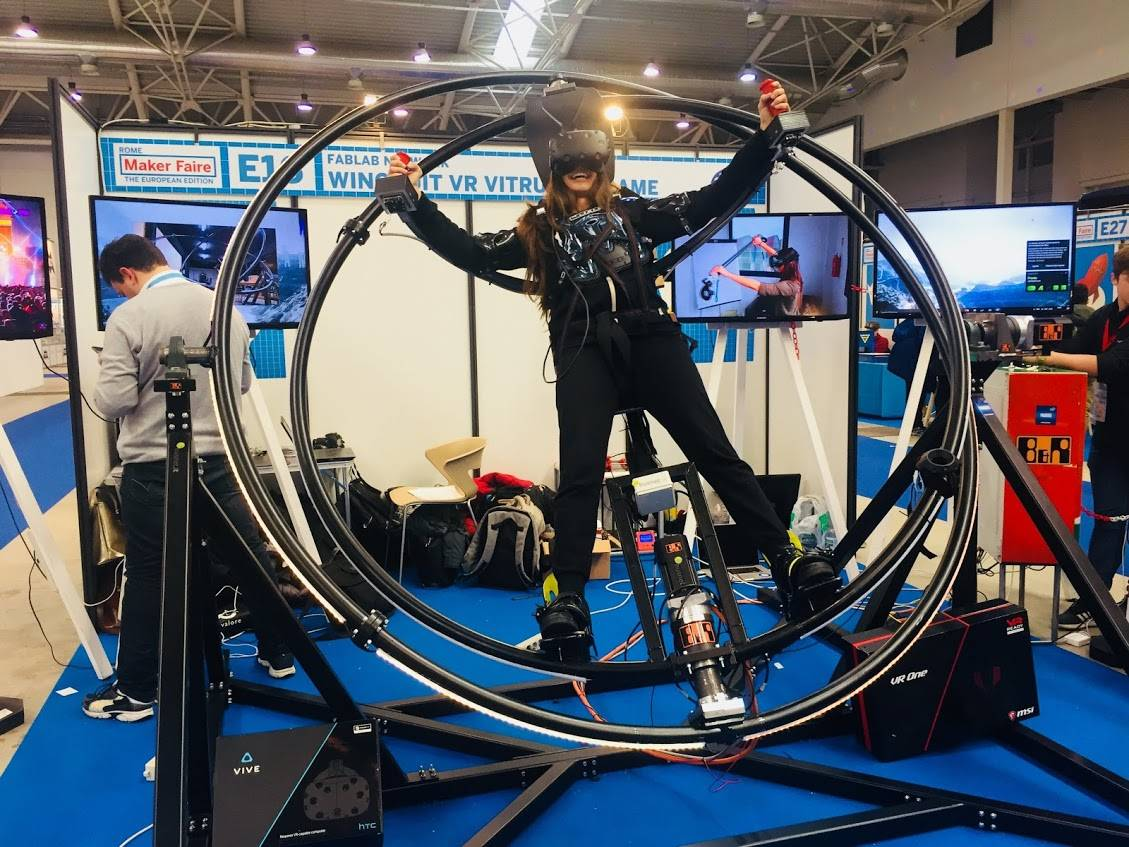
\includegraphics[scale=0.15]{immagini/vitruvian.jpg}
	\caption{Vitruvian Game - Il simulatore di volo con tuta alare}
	\end{center}
\end{figure}

\noindent \textbf{FabKey}
\\
FabKey è una serratura smart composta da un sistema di controllo connesso ad internet che permette l'apertura di una porta andando a verificare una lista di accessi presente in cloud. Funziona tramite tag \gls{NFC} o barcode. Il prodotto è rivolto principalmente ai \gls{FabLab}, ma si adatta facilmente a qualsiasi contesto in cui sia richiesto il controllo degli accessi.\\
Le principali tecnologie utilizzate in questo prodotto sono Arduino e relativa programmazione in Java per la parte hardware, mentre per il software crm sono stati utilizzati linguaggi come Html, Javascript, NodeJS, CSS ecc.
\\
\begin{figure}[H]
	\begin{center}
	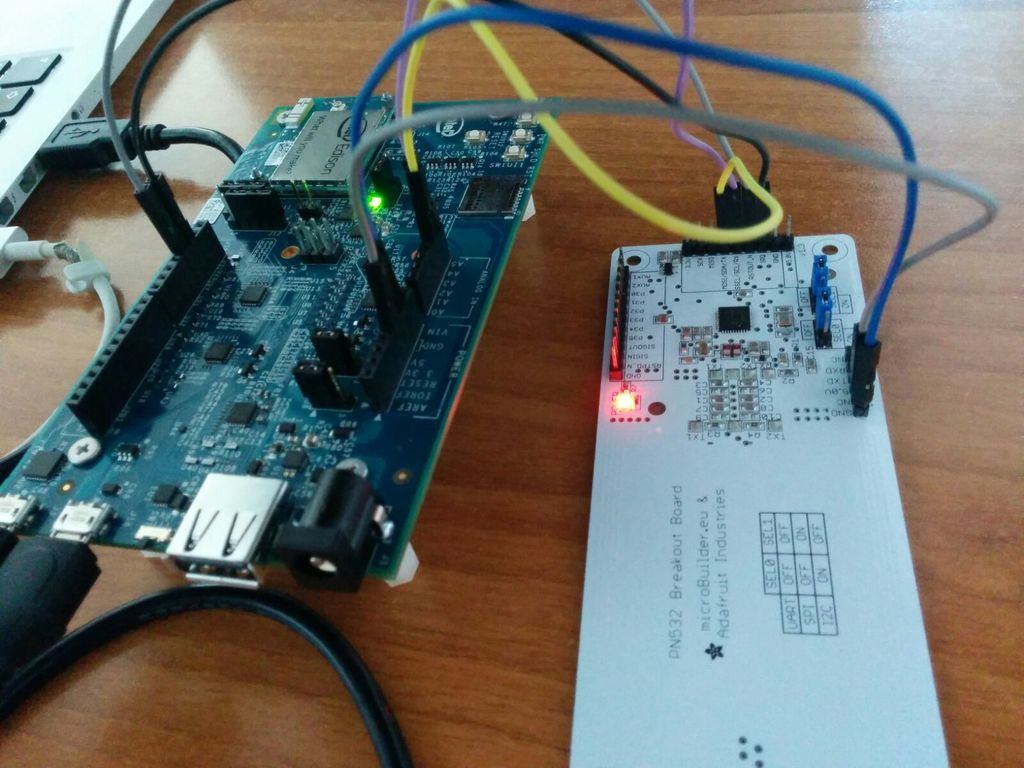
\includegraphics[scale=0.2]{immagini/fabkey.jpg}
	\caption{Prototipo di FabKey durante la fase di programmazione}
	\end{center}
\end{figure}

\noindent \textbf{Smart Meter}
\\
Un metro intelligente dotato di rotella metrica ed encoder ottico, capace di misurare superfici complesse e inviare direttamente i dati al software gestionale, in aggiunta anche il monitoraggio in tempo reale di quando, dove e per quanto tempo è stato utilizzato dal singolo addetto.\\
Il dispositivo è stato sviluppato sulla base di schede elettroniche programmabili open source.
\\
\begin{figure}[H]
	\begin{center}
	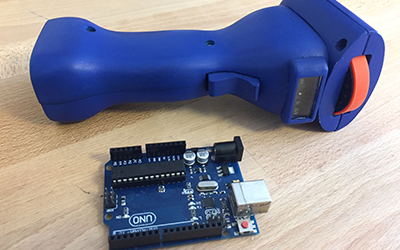
\includegraphics[scale=0.6]{immagini/smartmeter.png}
	\caption{Smart Meter: il metro intelligente}
	\end{center}
\end{figure}

\noindent \textbf{Progetti in via di sviluppo}
\\

\subsection{Servizi}
Il servizio principale che \lab{} offre ai propri clienti è quello di accompagnare le aziende in un percorso di aggiornamento tecnologico, fornendo supporto in termini di tecnologie e conoscenze.
L'iter che caratterizza questo servizio è il seguente:
\begin{itemize}
\item Analisi dettagliata delle esigenze del cliente;
\item Studio e progettazione della soluzione coinvolgendo le aziende partner che più si avvicinano alle materie trattate;
\item Implementazione dell'innovazione di processo o prodotto, lavorando in sinergia con le aziende selezionate.
\end{itemize}
Altri servizi che \lab{} offre ai propri clienti sono:
\begin{itemize}
\item \textbf{Didattica:} corsi di formazione su misura, \gls{counseling} e \gls{workshop} per imparare a sfruttare in modo professionale: stampa 3D, schede elettroniche, realtà virtuale e aumentata, sviluppo applicazioni, prototipazione, \gls{bigd}, \gls{iot} ecc.
\item \textbf{Noleggio:} kit e attrezzature come stampanti 3D, schede elettroniche (\gls{arduino}, \gls{rpi}, Intel) visori VR, pc e notebook, videoproiettori; affitto di aule didattiche;
\item \textbf{Personale qualificato:} per i clienti sono a disposizione docenti, tecnici di laboratorio e consulenti specializzati nei principali ambiti di innovazione digitale.
\end{itemize}

\subsection{Tecnologie}
L'intero team utilizza ambienti con sistema operativo \textit{macOS} per le attività di sviluppo. 
\subsubsection{Elettronica e Hardware}
A supporto dei processi di prototipazione, \lab{} utilizza diverse piattaforme hardware come ad esempio \textit{Arduino}, \textit{Raspberry Pi}, \textit{Intel UP Square}, \textit{Asus TinkerBoard}.\\
\lab{}, inoltre, sfrutta le potenzialità della stampa 3D e del disegno CAD per creare modelli prototipali in modo rapido. La disponibilità in azienda di 3 stampanti 3D permette di ridurre il tempo per la realizzazione dei prototipi da proporre al cliente.\\
Tali tecnologie sono state ampiamente utilizzate per lo sviluppo di progetti come FabKey e SmartMeter, soprattutto in fase di sperimentazione e prototipazione.

\begin{figure}[H]
	\begin{center}
	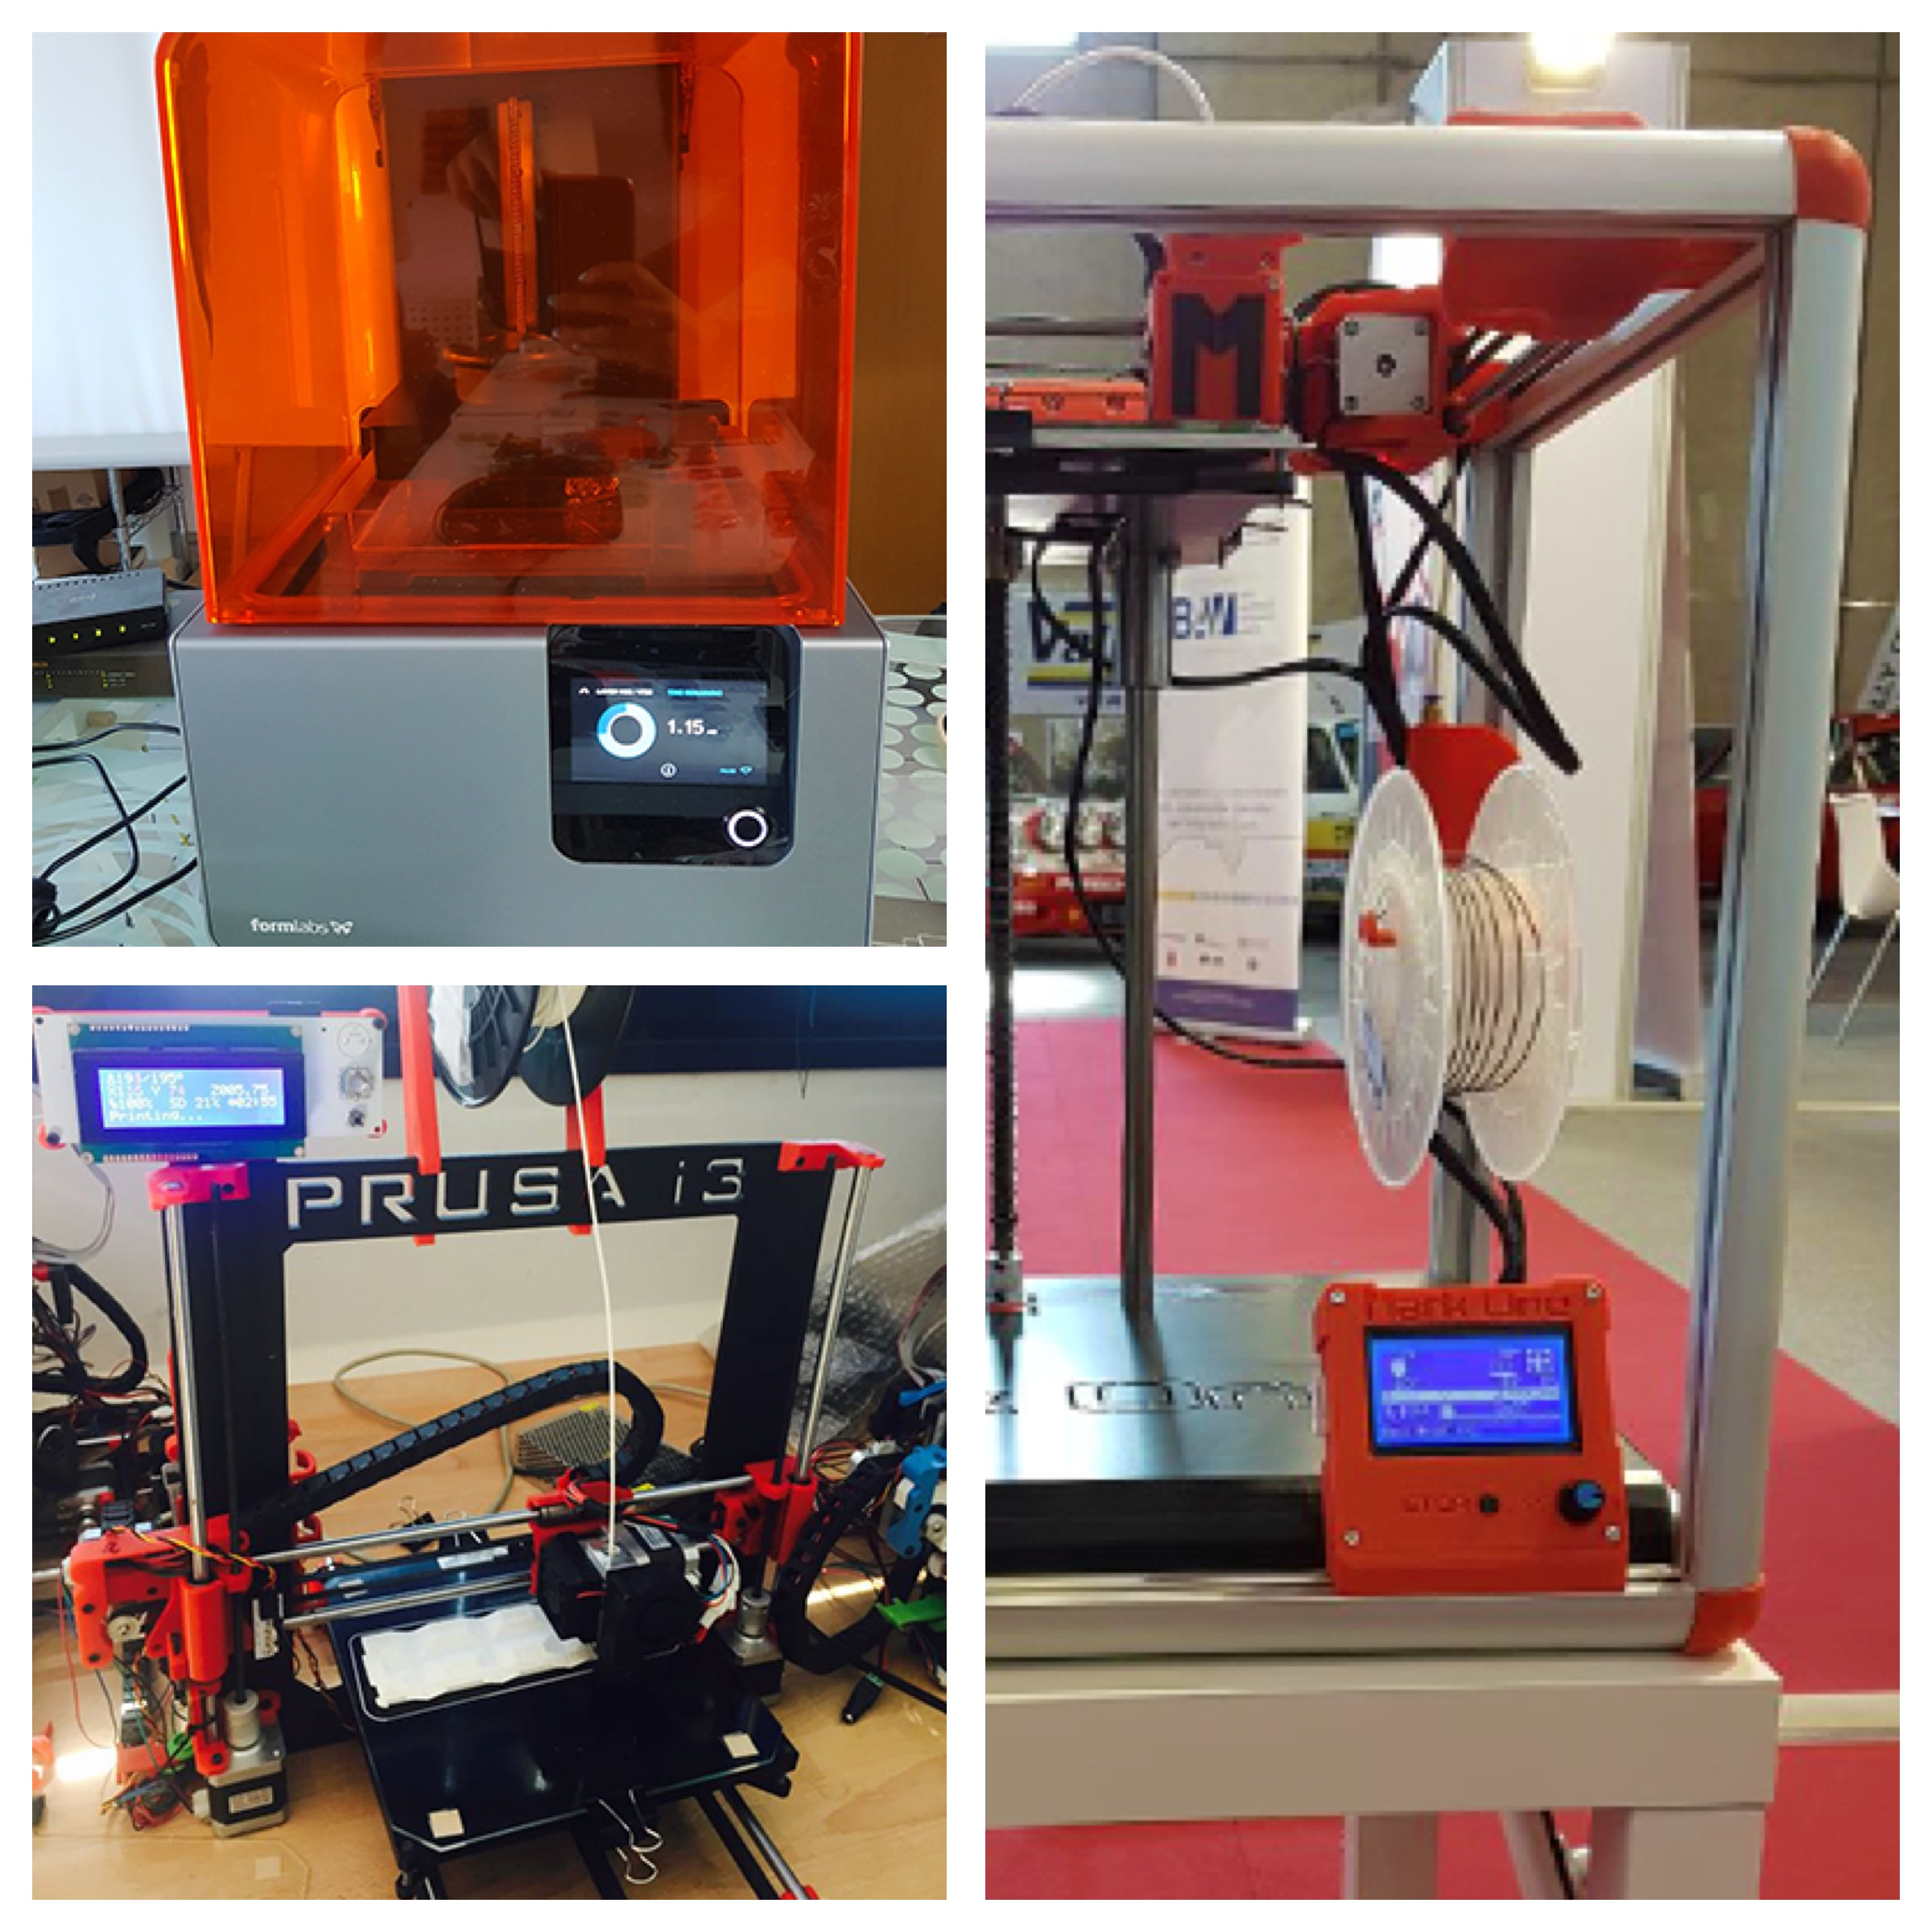
\includegraphics[scale=0.07]{immagini/stampanti.jpg}
	\caption{Le stampanti 3D in dotazione a \lab{}}
	\end{center}
\end{figure}

\subsubsection{Realtà virtuale e aumentata}
L'azienda utilizza software e strumenti per lo studio e lo sviluppo in ambito della realtà virtuale ed aumentata.
Nel dettaglio, è stato utilizzato il motore grafico \textit{Unreal Engine} per lo sviluppo dell'ambiente virtuale relativo al Vitruvian Game: per utilizzare e testare tale ambiente, \lab{} utilizza il visore \textit{Vive} prodotto da \textit{HTC}.\\
L'azienda, in ambito di realtà aumentata, utilizza la piattaforma \textit{Unity} per lo sviluppo di nuove applicazioni.\\

\subsubsection{Tecnologie di supporto}
A supporto dei processi di sviluppo, l'azienda utilizza la piattaforma web di \textit{GitLab}, che consente la gestione di repository Git e di funzioni trouble ticket.\\
L'utilizzo di questa piattaforma permette il controllo della configurazione e del versionamento di un software, oltre che la gestione di ticket.

\subsubsection{Applicazioni mobile}
Per lo sviluppo di applicazioni mobile, sia Android che iOS, \lab{} utilizza gli ambienti di sviluppo \textit{Android Studio} e \textit{Xcode}.
\\I linguaggi di programmazione utilizzati sono:
\begin{itemize}
\item Android Studio
	\begin{itemize}
		\item Java
	\end{itemize}
\item Xcode
	\begin{itemize}
		\item C++
		\item C
		\item Swift
		\item Objective-C
	\end{itemize}
\end{itemize}

\subsubsection{Deep Learning e intelligenza artificiale}
Utilizzando Intel Movidius, \lab{} sta attualmente sviluppando un progetto che consiste nella previsione di futuri incidenti e infortuni sul lavoro.\\
Sfruttando le tecniche di \textit{deep learning} messe a disposizione dall'hardware, si è in grado, analizzando grandi dati riguardanti incidenti passati, di effettuare una stima sui possibili incidenti futuri.

\section{Lab Network e innovazione}
\lab{} si è sviluppata nell'ambito della \textit{smart specialisation} attraverso logiche di coinvolgimento di una comunità di utenti misti che provengono prevalentemente dal mondo aziendale e accademico. 
L'azienda si propone come punto di riferimento per l'innovazione \textit{Open Source} nel territorio del Veneto, tramite la rete interconnessa dei \gls{FabLab} esistenti, e promuovendosi come centro privilegiato di interscambio di conoscenza.\\
Comprendendo che il tessuto imprenditoriale veneto è composto quasi totalmente di piccole e medie imprese dinamiche ed interconnesse, con un'industrializzazione diffusa ed una forte vocazione di tipo manifatturiero, \lab{} si è posta l'obiettivo di contribuire, attraverso strumenti e modalità di funzionamento specifici, a sviluppare ed attuare la strategia Regionale della ``Fabbrica Intelligente Del Futuro''.\\
Questa mira ad indirizzare la trasformazione del settore manifatturiero verso nuovi prodotti, processi e tecnologie, attraverso lo sviluppo di attività di ricerca di alto livello.

\subsection{Smart Specialisation Strategy}
\begin{figure}[H]
	\begin{center}
	
\includegraphics[scale=0.4]{immagini/join-s3p.png}
	\caption{Logo della piattaforma della Smart Specialisation.}
	\small{\textbf{Fonte:} \url{http://s3platform.jrc.ec.europa.eu}}
	\end{center}
\end{figure}

La \textit{Smart Specialisation} è una strategia concepita nell'ambito della politica di coesione riformata dalla Commissione Europea.\\
La specializzazione intelligente è un approccio fondato sull'individuazione di aree strategiche di intervento, basate sia sull'analisi dei punti di forza e del potenziale dell'economia sia su un processo di scoperta imprenditoriale con ampio coinvolgimento delle parti interessate.\\
Abbraccia un'ampia visione dell'innovazione, inclusi, ma certamente non limitati a, approcci incentrati sulla tecnologia e supportati da efficaci meccanismi di monitoraggio.\\
\\
Attraverso il portale dedicato che \lab{} utilizza per scambiare informazioni, le aziende e i makers possono lavorare in autonomia, ma condividendo le informazioni che possono essere attinte per le attività che competono a più soggetti.\\
\\
L'\gls{SWOT} sulla realtà delle PMI venete, contenuta nella Smart Specialisation Strategy, evidenzia come ci sia uno scarso utilizzo di tecnologie ICT, scarsa disponibilità di laboratori di proprietà, bassi investimenti in ricerca, difficoltà a sviluppare progetti innovativi e ridotta capacità di reperire risorse e professionalità necessarie. 
L'obiettivo di \lab{} è quello di colmare queste lacune mettendo a disposizione alle azienda un'area di lavoro a costi contenuti dove poter utilizzare i principali strumenti di innovazione digitale come: stampanti 3D, kit elettronici, macchine a controllo numerico, frese digitali e taglio laser. Tutto questo può essere definito come un laboratorio per studiare la fase prototipale.
\\
In pratica \lab{} vuole contribuire a portare l'innovazione e la tecnologia all'interno delle PMI che ancora non si sono interfacciate a questo ''nuovo mondo``.

